%!TEX root = main.tex
\onehalfspacing
315 subjects from 19 countries participated in this study. Of the 315 test subjects, 112 (66 male / 46 female) finished the questionnaire. This corresponds to a completion rate of 40.79\%. The age of the subjects ranged from 19 to 46 with an average age of approximately 28 years. \par

\begin{table}[!ht]
	\centering
	\begin{tabu} spread 20pt {c c c c c }\toprule
	% & \multicolumn{6}{c}{Formulations}  \\ \cmidrule{2-7}
Total	&Male	&Female&	Experimental Group&	Control Group\\ \midrule
112     &	66  &	46 &	72                &	40\\
100.00\%& 58.93\%&	41.07\%&	64.29\%&	35.71\%\\ \bottomrule
	\end{tabu}
	\caption{Random sample of the participants before the adjustment distinguished by ‘gender’ and experimental / control group.}
	\label{tab:gender}
\end{table}
However, due to significant mistakes and deviation of the average and anticipated perfor-mance time, the participants’ number was adjusted to a total of 86.  \par
The experiment was based on a two factorial between the distinguishing mark (depletion and non-depletion) designs. The main dependent measure was social risk in decision-making. The decision-making served as a measurement of social risk tendencies. The adjusted sample consisted of (\res{N~=~86}) participants (33 male / 53 female) aged between 20 and 46 (\res{M~=~28.151; SD~=~5.13}). The experimental group consisted of (\res{N~=~30}) participants  (13 male / 17 female) and the control group consisted of (\res{N~=~56}) participants (20 male / 36 female).\par
The experiment was designed as an online questionnaire study. Its first aim was to provide the participants with the opportunity for self-evaluation in the context of consumer, spending and risk behaviour. After answering the self-evaluation part, the participants were randomly assigned to two groups. Group 1 (experimental group) had to accomplish a ‘Stroop test’, containing three sets of 60 questions each. The experimental-condition task was designed to de-plete participants within approximately 15 to 20 minutes. The task used for the control group was identical to the one used in the experimental condition but did not include the depletion measure. Therefore, all words were presented in dark grey (see above), so that a depletion of the control group was not expected. After completing the task, participants were instructed to decide between two alternatives of a product, which could be distinguished by one attribute only (e.g. colour). Figure \ref{fig:os_product_choice} depicts an example of the decision making task of the questionnaire. \par

\begin{figure}[h!]
\center
	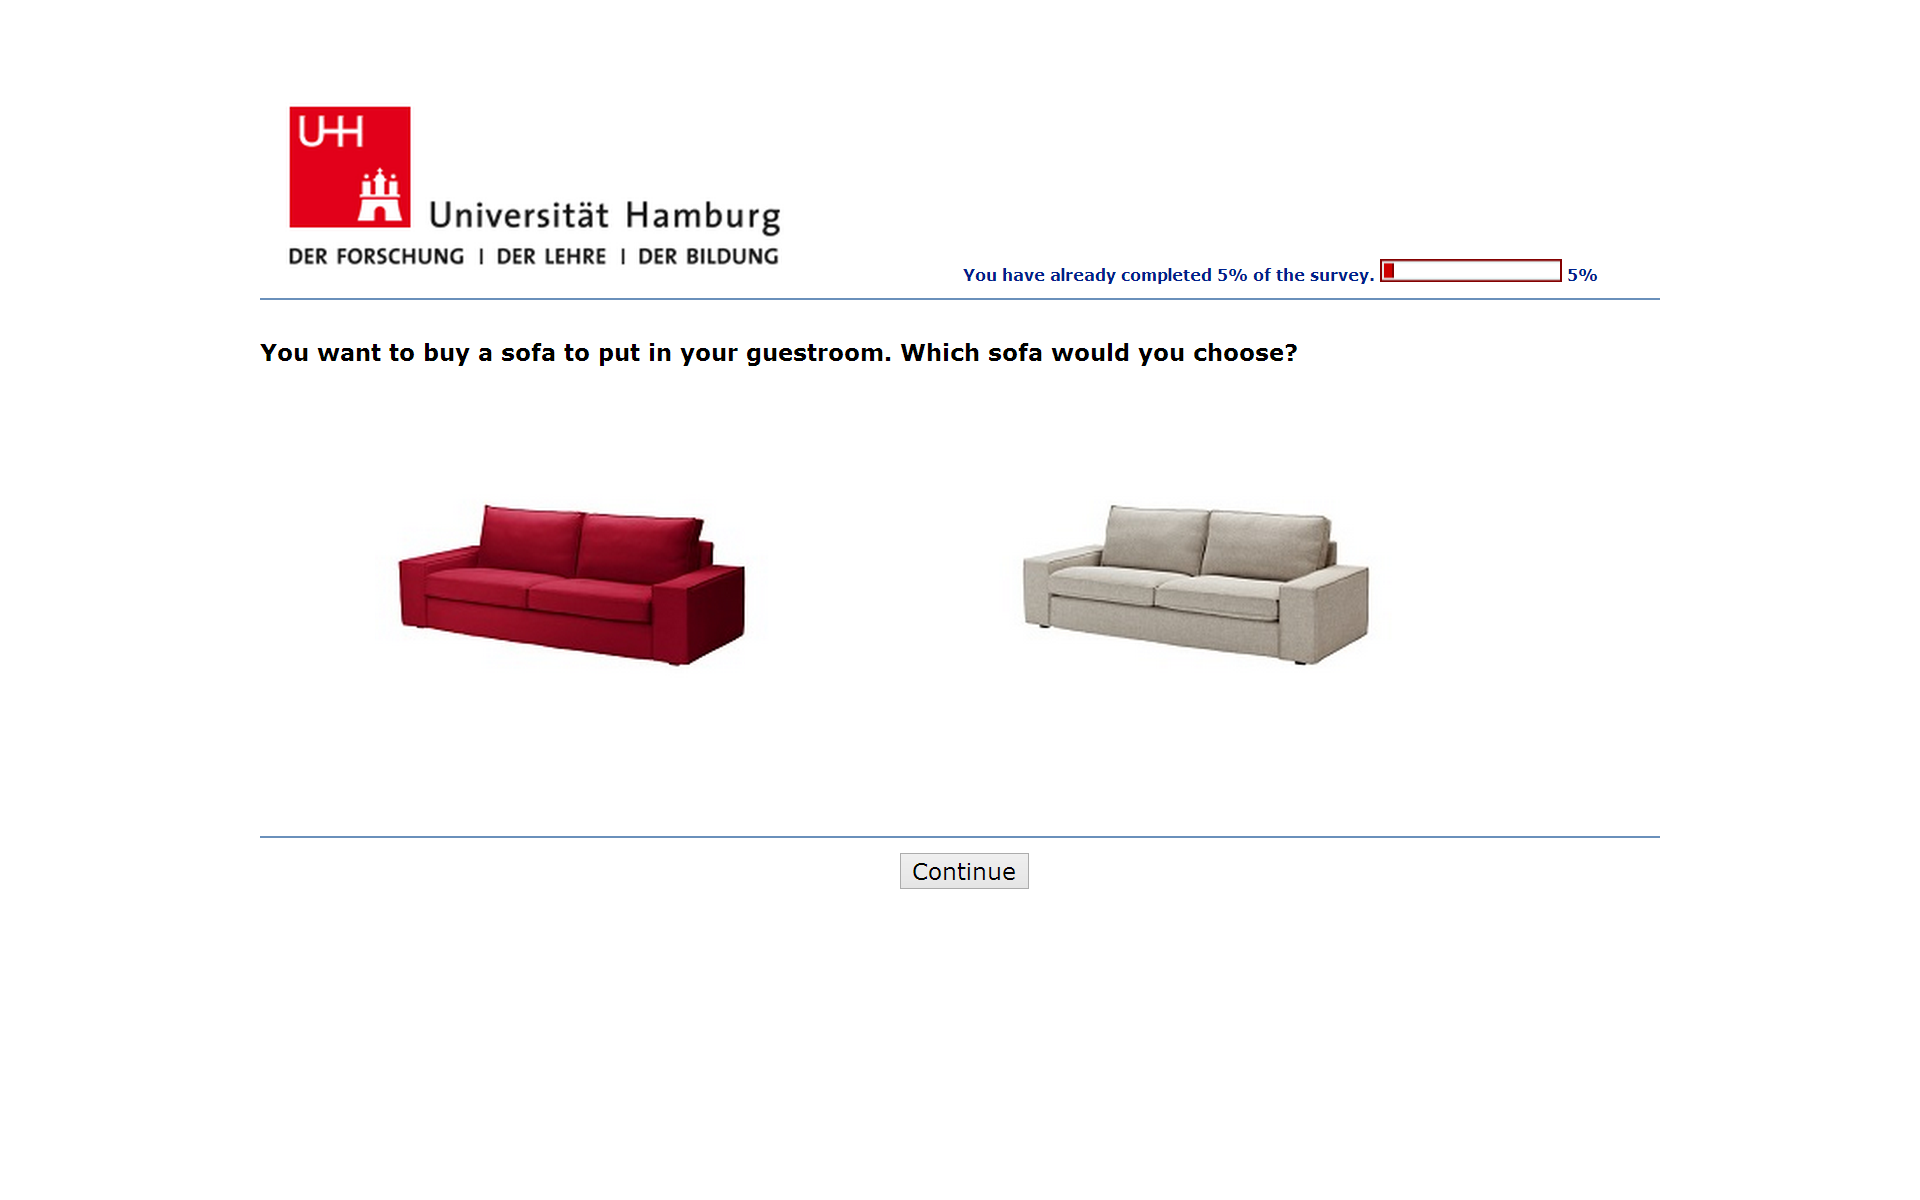
\includegraphics[trim= 0pt 8cm 0pt 2cm, clip=true,width=0.9\textwidth]{images/os_product_choice.png}
  \caption{Example of product choice in online questionnaire (sofa)}\label{fig:os_product_choice}
\end{figure}
By putting the decision in a situation of a social context ‘You want to buy a sofa to put in your guestroom’, we tried to emphasize the social contribution ‘people will see this item that I bought and might judge me on the basis of this purchase’. Each product was placed in a dif-ferent social framework\footnote{In order not to violate any trademark rights, the brands in the online questionnaire have been removed. However, some of the products posses a high recognition factor and might influence the participants after all.}. After the decision-making task based on purchases the questionnaire proceeded with questions based on the judges’ dilemma (compare Chapter \ref{sec:consumerchoice}). Before the participants could finalize their decision they were informed that their verdict as to whether the perpetrator would be granted probation or if he/she would remain in custody was crucial. They were also asked to keep in mind that while resocialization is an important objective, so is keeping in custody a possible repeater. Both tasks regarding decision-making were aimed at generating an environment of social risk. After the decision-making task participants were instructed to answer questions in order to examine the degree of their depletion (see Chapter \ref{sec:consumerchoice}). Subsequently participants were asked to state their perceived level of exhaustion on a Likert scale (ranging from ‘not at all exhausted’ to ‘very exhausted’) and how they assessed the level of difficulty regarding the Stroop test (ranging from ‘very easy’ to ‘very difficult’).\par

\section{Analysis of Group Differences}
In the following section the collected data of the questionnaire will be presented. To test the hypothesis (difference in decision-making under the influence of social risk between control group and experimental group), we analyzed whether the independent variable ‘ego deple-tion’ affected the participants’ preference for the low social risk option. In order to ensure that the two groups did not differ from each other in any important aspect a priori, which might account for manipulations of the data, we considered it important to conduct a series of tests, which will be presented in detail beforehand.\par
In order to ensure that participants’ gender was no interfering variable a chi-squared test was administered.  The experimental group and the control group did not show any distinctive difference regarding the variable ‘gender’ (\res{x\textsuperscript{2} = 0.49; df =1; p = 0.49}).  \par

\begin{table}[!ht]
	\centering
	\begin{tabu} spread 20pt {r|X[1,c] X[1,c]| c }\toprule
	% & \multicolumn{6}{c}{Formulations}  \\ \cmidrule{2-7}
	Groups   & female & male &Total\\ \midrule
	non-depl &  36    & 20   &56\\
	depl     &  17    & 13   &30\\ \midrule
	Total    &  53    & 33   &86\\ \bottomrule
	\end{tabu}\\ \vspace{8pt}
	\begin{tabu} spread 20pt {l r}
	Pearson chi\textsuperscript{2}(1) =   0.4795&  Pr = 0.489\\
	\end{tabu}
	\caption{Results of the chi-squared test in regard to ‘gender’ and the ‘depletion’/’non-depletion’ condition.}
	\label{tab:gender}
\end{table}

In order to ensure that participants’ age was no interfering variable a two-sample t-test with equal variance with the variable (age) in the experimental group (\res{N = 30; m = 28.833; SD = 4.913}) and the control group (\res{N = 56; m = 27.785; SD = 5.249}) was administered. As expected, it did not show any distinctive difference between the variances (\res{t = -0.91; df(84); p = 0.9096}). Therefore, we conclude that the mean is statistically not significantly different from zero. \par

\begin{table}[!ht]
	\centering
	\setlength{\tabcolsep}{1.2em}{
	\begin{tabu} spread 20pt {r|c c c c c}\toprule
	% & \multicolumn{6}{c}{Formulations}  \\ \cmidrule{2-7}
	    Variable &       Obs    &    Mean &   Std. Dev.  &     Min    &    Max\\
\midrule %-------------+--------------------------------------------------------
      Time1  &        86 &   167.8488 &    59.0586 &        93  &      358\\
% \midrule %-------------+--------------------------------------------------------
      Time2  &        86 &   147.7326 &   31.07199 &        94  &      290\\
% \midrule %-------------+--------------------------------------------------------
      Time3  &        86 &  145.7442  &  32.31725  &       94   &      296\\ \bottomrule
	\end{tabu}}\\
	\caption{Stroop test displays the variable Time1, Time2, Time3 with the corresponding  observation, mean, standard deviation, minimum and maximum period of time.}
	\label{tab:stroop_time}
\end{table}

During the depletion task (Stroop test) the participants had 30 seconds to answer each question (compare Table \ref{tab:stroop_time}). An exceedance of the specified time limit automatically lead to the termination of the questionnaire.  The variable ‘time’ aims at the time needed by the participants for the Stroop test. Although a strong difference regarding the standard deviation between the variable Time 1 (required time to finish the first Stroop test) (\res{SD = 59.06}) and the variables Time 2 (required time to finish the second Stroop test) (\res{SD =  31.07}) and Time 3 (required time to finish the third Stroop test) (\res{SD = 32.32}) was observed, it can be explained by the assumption of an adaption phase for the participants. It appears that after a short period of time participants adjusted to the test.\par
A two-sample t-test was conducted in order to check whether the variable time differed significantly between participants in the non-depletion and the depletion condition. Surprisingly, the test did not reveal any significant difference in means regarding the variable (time) between the experimental group and the control group (\res{t = -6.91; df = 84; p = 0.000}) A possible explanation could be that the given time limit prevented any major differences between the groups. \par
The variable ‘correct answers’ shows the number of correct answers given by the partici-pants in the Stroop test. A minimum of 30 (of a total of 60) correct answers per set was necessary to be included into the evaluation. This limit was imposed because it was assumed that no or only little depletion would occur below that threshold, in any case not enough for our purposes. The results appear to comply with the assumption that some participants would need some time to adjust to the task at hand. \par
While the means of Stroop 1, 2, and 3 do not revealingly differ from each other (\res{mStroop1 =57.44; mStroop2 = 58.22; mStroop3 = 58.22}), a difference regarding the standard deviation (\res{SD = 4.58}) of Stroop 1 (correct answers in the first Stroop test) to the standard deviation (\res{SD = 3.62}) Stroop 2 (correct answers in the second Stroop test) emerged. Nevertheless, this was not the case between Stroop 2 and Stroop 3 (\res{SD = 3.77}) (compare Table \ref{tab:stroop_stroop}). A possible explanation accounting for this difference is the previously hypothesized adaption phase for the participants.\par

\begin{table}[!ht]
	\centering
	\setlength{\tabcolsep}{1.2em}{
	\begin{tabu} spread 20pt {r|c c c c c}\toprule
	    Variable &       Obs    &    Mean &   Std. Dev.  &     Min    &    Max\\ \midrule
		Stroop1&        86&    57.44186 &   4.575137  &       38 &        60\\
		Stroop2&        86&    58.22093 &   3.615005  &       44 &        60\\
		Stroop3&        86&    58.22093 &   3.771101  &       40 &        60\\ \bottomrule
	\end{tabu}}\\
	\caption{Stroop test displays the variable Stroop1, Stroop2, Stroop3 with the corresponding observation, mean, standard deviation, minimum and maximum of correct answers.}
	\label{tab:stroop_stroop}
\end{table}

\section{Data Reduction and Analysis of Group Differences}\label{sec:factoranalysis}
\subsection{General Self-Control}

Table 6 shows the items of the General Self-Control scale  (SCS) and their corresponding statements used in the questionnaire. The variables Item 1 and Item 5 had to be adjusted for the factor analysis, as they were reverse coded. 

\begin{table}[!ht]
	\centering
	\setlength{\tabcolsep}{1.2em}{
	\begin{tabu} spread 20pt {l l}\toprule
	General Self-Control scale&	Item -  Statement\\ \midrule
	GSC1&	I never allow myself to loose control.\\
	GSC2&	I am not easily discouraged.\\
	GSC3&	I am good at resisting temptation. \\
	GSC4&	I have worked or studied all night at the last minute.\\
	GSC5&	I have a hard time breaking bad habits.\\ \bottomrule
	\end{tabu}}\\
	\caption{General Self-Control scale and the corresponding statements. }
	\label{tab:selfcontrol}
\end{table}

To check if the many different statistical variables of the questionnaire on self-control underly a few latent variables, a factor analysis using a varimax rotation was performed. Table \ref{tab:factorloading} displays the factor loadings, indicating the relation among the GSC items. While Items 1, 2 and 5 loaded on the first factor, Items 3 and 4 loaded on the second factor (see Table \ref{tab:factorloading}). Cronbach’s alpha was also assessed ($\alpha$\res{ = 0.55}) but did not reveal any significant internal consistency of the GSC (see Table \ref{tab:cronbachalpha}). Consequently, it appears that the items of the GSC should not be merged into one latent variable, as intended in the first place. It is possible that the reduction of the questionnaire, which originally contained 36 items, might have led to these results. This will be discussed at a later point.\par

\begin{table}[!ht]
	\centering
	\setlength{\tabcolsep}{1.2em}{
	\begin{tabu} spread 20pt {l c c c c}\toprule
        Variable &  Factor1 & Factor2 & Factor3 &  Uniqueness \\ \midrule
    
            GSC1 &  \textbf{0.6615} & -0.0027  &  0.0784 &      0.5562 \\ 
            GSC2 &   \textbf{0.6910} & 0.2886   & -0.0314 &      0.4382 \\ 
            GSC3 &   0.2396  & \textbf{0.5489}  &  0.0095 &      0.6412 \\ 
            GSC4 &   0.1106  & \textbf{0.3121}  &  0.1659 &      0.8629 \\ 
            GSC5 &   \textbf{0.2854}  &  0.0488  &  0.0397 &      0.9146 \\ \bottomrule
    
	\end{tabu}}\\
	\caption{Results of the orthogonal rotated factor loadings (General Self-Control). Highest factor loading in bold displayed.}
	\label{tab:factorloading_gsc}
\end{table}
\begin{table}[!ht]
	\centering
	\setlength{\tabcolsep}{1.2em}{
	\begin{tabu} spread 20pt {X[l] X[0.5,l] X[0.2,c] X[2.7,c] X[2.7,c] X[3,c] X[c] }\toprule                                    
Item         &  Obs & Sign &  item-test correlation &  item-rest correlation & average interitem covariance & alpha \\ \midrule
GSC1        &   86  &  $+$  &    0.6145  &   0.3862  &  .2030096 &  0.4629 \\
GSC2        &   86  &  $+$  &    0.7204  &   0.5011  &   .148404 &  0.3854 \\
GSC3        &   86  &  $+$  &    0.6068  &   0.3379  &  .2064067 &  0.4827 \\
GSC4        &   86  &  $+$  &    0.5148  &   0.1981  &  .2584587 &  0.5635 \\
GSC5        &   86  &  $+$  &    0.5695  &   0.2076  &  .2428865 &  0.5738  \\ \midrule
Test scale  &       &     &            &           &  .2118331 &  0.5521 \\ \bottomrule

	\end{tabu}}\\
	\caption{Result of Cronbachs alpha analysis (General Self-Control). Result displays the item-test correlation, item-rest correlation, the average interitem covariance and the alpha value.}
	\label{tab:cronbachalpha_gsc}
\end{table}
Table \ref{tab:scoregsc} shows a comparison of the mean (score GSC) between the depletion and the non-depletion group. As the factor analysis did not produce the desired results, a two-sample t-test with equal variances of each item of the General Self-Control Scale had to be performed, again, this was done to ensure that there was no difference between the groups, which might act as an interfering variable. As expected, this procedure did not produce any evidence that the experimental group and the control group differed significantly in their means (\res{t = -0.21; -1.50; -1.54; -1.53; -0.42; df = 84; $\alpha$ < 0.05}) (see Table \ref{tab:scoregsc}). 

\begin{table}[!ht]
	\centering
	\setlength{\tabcolsep}{1.2em}{
	\begin{tabu} to 440pt {X[2.2,l] X[c] X[c] X[c] X[c] X[2.5,c] X[5,c] }\toprule                                    
Item        &  M (depl) & M (non-depl) &  SD (depl)	 &  SD (non-depl) &   Two tailed p-value & t (df)\\ \midrule

GSC1 &	4.667 &	4.625	& 0.758	& 0.945	 & 0.84	& t(df =84)= -0.21 \\ 
GSC2 &	3.100 & 2.768	& 1.062	& 0.934	 & 0.14	& t(df =84)= -1.50 \\
GSC3 &	3.434 &	3.089	& 1.006	& 0.978	 & 0.13	& t(df =84)= -1.54 \\
GSC4 &	3.667 &	3.304	& 0.959	& 1.094	 & 0.13	& t(df =84)= -1.53 \\
GSC5 &	4.634 &	4.518	& 0.217	& 0.167	 & 0.68	& t(df =84)= -0.42 \\ \bottomrule
	\end{tabu}}\\
	\caption{Summary of the General Self-Control results of the two-sample t-test with equal variances. The table displays the means and the standard deviation of the depletion and the non-depletion group and the two-tailed p-value, t-value and the degrees of freedom.}
	\label{tab:ttest_scoregsc}
\end{table}

\subsection{Exploratoy Tendencies in Consumer Behaviour}

Table \ref{tab:exploratoryscale} shows the itmes of the Exploratory Tendencies in Consumer Behaviour scale  (CBS) and their corresponding statements used in the questionnaire. 
\begin{table}[!ht]
	\centering
	\setlength{\tabcolsep}{1.2em}{
	\begin{tabu} to 440pt {X[0.2l] X[l]}\toprule
	     Item &	Item - Statement \\ \midrule
	CBS1	& I often delay taking action until I have carefully considered the consequences of my purchase decisions.\\
	CBS2	& I am responsible when it comes to how much I spend.\\
	CBS3	& When I go out with my friends, I keep track of what I am spending.\\
	CBS4	& I closely monitor my spending behavior.\\ \bottomrule
	\end{tabu}}\\
	\caption{Exploratory Tendencies in Consumer Behaviour items and the corresponding statements.}
	\label{tab:cbs_scale}
\end{table}
To check if the many different statistical variables of the questionnaire on consumer behaviour, underly a few latent variables, a factor analysis using a varimax rotation was performed. Table 11 displays the factor loadings, indicating the relation among the CBS items. While Items 1, 3 and 4 loaded on the first factor, Item 2 loaded on the second factor. Cronbach’s alpha was also assessed ($\alpha$\res{ = 0.30}) and did not reveal any internal consistency of the CBS (see Table \ref{tab:cronbach_alpha_cbs}). Again, consistent with the findings on the GSC, it appears that the items of the CBS should not be merged into one latent variable, as was expected following the original data (see \cite{raju1980optimum}). Again, it is possible that the reduction of questionnaire, which originally contained 39 items, might have led to these results. This will be discussed at a later point.
\begin{table}[!ht]
	\centering
	\setlength{\tabcolsep}{1.2em}{
	\begin{tabu} spread 20pt {l c c c }\toprule
        Variable &  Factor1 & Factor2 & Uniqueness \\ \midrule
            CBS1 &   0.0218 &   \textbf{0.1991} &   0.9599 \\ 
            CBS2 &  -0.5448 &  \textbf{-0.0241} &   0.7026 \\ 
            CBS3 &   \textbf{0.3090} &  -0.0308 &   0.9036 \\ 
            CBS4 &   \textbf{0.4515} &  -0.0614 &   0.7923   \\ \bottomrule

	\end{tabu}}\\
	\caption{Results of the orthogonal rotated factor loadings (CBS). Highest factor loading in bold displayed.}
	\label{tab:rotated_factor_cbs}
\end{table}
\begin{table}[!ht]
	\centering
	\setlength{\tabcolsep}{1.2em}{
	\begin{tabu} spread 20pt {X[l] X[0.5,l] X[0.2,c] X[2.7,c] X[2.7,c] X[3,c] X[c] }\toprule                                    
Item         &  Obs & Sign &  item-test correlation &  item-rest correlation & average interitem covariance & alpha \\ \midrule

CBS1         &  86 &  $+$  &   0.4958  &   -0.0069  &    .655586  & 0.4539\\
CBS2         &  86 &  $-$  &   0.6768  &    0.3669  &  -.0063383  &      .\\
CBS3         &  86 &  $-$ &   0.5425  &    0.1342  &   .3580027  & 0.2601\\
CBS4         &  86 &  $-$ &   0.5854  &    0.1775  &   .2692658  & 0.2072\\ \midrule
Test scale   &     &      &           &            &    .319129  & 0.2962\\ \bottomrule

	\end{tabu}}\\
	\caption{Result of Cronbach’s alpha analysis (CBS). Result displays the item-test correlation, item-rest correlation, the average interitem covariance and the alpha value.}
	\label{tab:cronbach_alpha_cbs}
\end{table}

Table \ref{tab:mean_comparison} shows a comparison of the mean (score CBS) between the depletion and the non-depletion group. As the factor analysis did not produce the expected results, a two-sample t-test with equal variances of each item of the Exploratory Tendencies in Consumer Behaviour Scale had to be performed for reasons stated above. As expected, this procedure did not pro-duce any evidence that the experimental group and the control group differed significantly in their means (\res{t = -0.70; 0.51; 0.81; -0.80; df = 84; $\alpha$ < 0.05}) (see Table \ref{tab:mean_comparison}). 

\begin{table}[!ht]
	\centering
	\setlength{\tabcolsep}{1.2em}{
	\begin{tabu} to 440pt {X[2.2,l] X[c] X[c] X[c] X[c] X[2.5,c] X[5,c] }\toprule                                    
Item        &  M (depl) & M (non-depl) &  SD (depl)	 &  SD (non-depl) &   Two tailed p-value & t (df)\\ \midrule

CBS1 &	3.634 &	3.304	& 1.991 &2.140	& 0.49	& t(df =84)= -0.70 \\
CBS2 &	4.100 &	4.286	& 1.668 &1.581	& 0.61	& t(df =84)=  0.51 \\
CBS3 &	3.334 &	3.661	& 1.826 &1.761	& 0.42	& t(df =84)=  0.81 \\
CBS4 &	4.900 &	4.571	& 1.845 &1.818	& 0.43	& t(df =84)= -0.80 \\ \bottomrule

	\end{tabu}}\\
	\caption{Summary of the Exploratory Tendencies of Consumer Behaviour results of the two-sample t-test with equal variances. The table displays the means and the standard deviation of the depletion and the non-depletion group and the two tailed p-value, t-value and the degrees of freedom.}
	\label{tab:mean_comparison}
\end{table}
\subsection{Consumer Spending Self-Control}\label{sec:consumer_spending_self_control}
Table \ref{tab:consumerspendingselfcontrol} depicts the items of the Consumer Spending Self-Control Scale  (SSC) and their corresponding statements used in the questionnaire. The items 1 and 4 had to be adjusted, as they were reverse coded. 

\begin{table}[!ht]
\tabulinesep=1.8mm{
	\centering
	\setlength{\tabcolsep}{1em}{
	\begin{tabu} to \textwidth {X[l] X[2.8,l]}\toprule
	Item	&Item - Statement\\ \midrule
SSC1&	Even though certain food products are available in a number of different flavors, I always tend to buy the same flavor.\\
SSC2&	When I see a new brand somewhat different from the usual, I investigate it.\\
SSC3&	A new store or restaurant is not something I would be eager to find out about.\\
SSC4&	When I see a new or different brand on the shelf, I often pick it up just to see what it is like.\\ \bottomrule
	\end{tabu}}\\
	\caption{Consumer Spending Self-Control items and the corresponding statements.}
	\label{tab:consumerspendingselfcontrol}}
\end{table}
To check if many different statistical variables of the questionnaire on consumer spending, underly a few latent variables, a factor analysis using a varimax rotation was performed. Table \ref{tab:rotated_factor_loading_consumer_spending_selfcontrol} displays the factor loadings, indicating the relation among the CSSC items. This time, all items loaded on a single factor. Cronbach’s alpha was also assessed (\res{$\alpha$ = 0.80}) confirming a significant internal consistency of the SSC items (see Table \ref{tab:cronbach_alpha_consumer_spending_self_control_scale}). 
\begin{table}[!ht]
	\centering
	\setlength{\tabcolsep}{1.2em}{
	\begin{tabu} spread 20pt {l c c }\toprule
     
     Variable &  Factor1 & Uniqueness \\ \midrule
            SSC1 &  0.6289 &  0.6045\\
            SSC2 &  0.7283 &  0.4695\\
            SSC3 &  0.6579 &  0.5672\\
            SSC4 &  0.7537 &  0.4319\\ \bottomrule
   

	\end{tabu}}\\
	\caption{Results of the orthogonal rotated factor loadings (SSC).}
	\label{tab:items_Exploratory_Tendencies_Consumer_Behaviour}
\end{table}
\begin{table}[!ht]
	\centering
	\setlength{\tabcolsep}{1.2em}{
	\begin{tabu} spread 20pt {X[l] X[0.5,l] X[0.2,c] X[2.7,c] X[2.7,c] X[3,c] X[c] }\toprule                                    
Item         &  Obs & Sign &  item-test correlation &  item-rest correlation & average interitem covariance & alpha \\ \midrule
SSC1         &  86 &   $+$  &     0.7497 &   0.5587  &   .6159143 &  0.7803\\
SSC2         &  86 &   $+$  &     0.8302 &   0.6573  &     .49772 &  0.7338\\
SSC3         &  86 &   $+$  &     0.7649 &   0.5791  &   .5966712 &  0.7711\\
SSC4         &  86 &   $+$  &     0.8261 &   0.6794  &    .529275 &  0.7238\\ \midrule
Test scale   &     &      &            &           &   .5598951 &  0.8029\\ \bottomrule

	\end{tabu}}\\
	\caption{Result of Cronbach’s alpha analysis (SSC). Result displays the item-test correlation, item-rest correlation, the average interitem covariance and the alpha value.}
	\label{tab:cronbach_alpha_consumer_spending_self_control_scale}
\end{table}

With the satisfactory results of preceding tests at hand all items of the SSC were merged into one variable and a two-sample t-test with equal variances was performed, comparing the mean (score SSC) of the depletion and the non-depletion group. 

\begin{table}[!ht]
	\centering
	\setlength{\tabcolsep}{0.83em}{
	\begin{tabu} spread \textwidth {r|r r r r r r}\toprule
		Group &  Obs & Mean  &  Std. Err.&  Std. Dev. & \multicolumn{2}{r}{[95\% Conf. Interval]}\\
		\midrule %---------------------------------------------------------------------------------
		non-depl &     56 &   3.200893 &   .1083786 &   .8110314 &   2.983697 &   3.418088\\
		depl     &     30 &   3.466667 &   .1579927 &   .8653615 &   3.143535 &   3.789798\\
		\midrule %--------------------------------------------------------------------------
		combined &     86 &   3.293605 &   .0900479 &   .8350694 &   3.114565 &   3.472644\\
		\midrule %--------------------------------------------------------------------------
		diff     &        &  -.2657738 &   .1878331 &            &  -.6393006 &    .107753\\ 
		\midrule[0pt]\midrule[0pt]\midrule[0pt]\midrule[0pt]\midrule[0pt]
		\multicolumn{3}{l}{diff = mean(0) - mean(1)} &  & \multicolumn{3}{r}{t =  -1.4149}\\
		\multicolumn{3}{l}{Ho: diff = 0}             &  & \multicolumn{3}{r}{degrees of freedom = 84}
	\end{tabu}
	}
	\vspace{8pt}
	\setlength{\tabcolsep}{2em}{
	\begin{tabu} spread \textwidth {@{}X[c] X[c] X[c]@{}}
	    Ha: diff < 0     &          Ha: diff != 0          &        Ha: diff > 0\\
	 Pr(T < t) = 0.0804  &       Pr(|T| > |t|) = 0.1608    &      Pr(T > t) = 0.9196
	\end{tabu}}
	\caption{Two-sample t-test with equal variances on Consumer Spending on Self-Control results. The table displays the means, the confidence interval, the two tailed p-value, t-value and the degrees of freedom.}
	\label{tab:ttestssc}
\end{table}
As expected, this procedure did not produce any evidence that the experimental group and the control group differed significantly in their means (\res{t = -1.41; df = 84; $\alpha$ < 0.05}).

\section{Hypothesis Testing}
\subsection{Pearson Chi-Squared (Products)}\label{sec:pearson_chi_products}
% \newlength{\mylength}
% \setlength{\mylength}{\widthof{100\%}}
% \the\mylength
In order to investigate if there were any statistically significant differences in decision-making regarding products with low versus high social risk between depleted participants and non-depleted participants, we conducted a series of chi-squared tests with ‘product lowrisk/highrisk’ as the dependent variable and ‘non-depletion/depletion’ as the independent variable. We expected that depleted participants would opt in favor of products involving a low social risk. For greater clarity, figures on the left depict the absolute numbers, whereas figures on the right depict the ratio.\par
Results regarding the product ‘sofa’ did not reveal a statistically significant relationship between condition and social risk (\res{Pearson chi\textsuperscript{2} (1)  = 0.7395; p = 0.390}) and in addition the result was converse to our expectation. In contrast to our expectations, 66\% of the non-depletion condition group opted for low risk, whereas 34\% opted for high risk. In the depletion condition group 57\% of the participants opted for low risk, whereas 43\% opted for high risk. As expected, both groups showed a clear preference for the low risk alternative although this preference was more pronounced within the non-depletion condition (see Figure 16). This result was not only unexpected but it also contradicts our initial assumption.\par
\begin{figure}[!h]
\begin{floatrow}
\capbtabbox{%
	\begin{tabu} spread 0pt {r|X[1,c] X[1,c]| c }\toprule
	   sofa    &   lowrisk &  highrisk &     Total\\ \midrule
	  non-depl &        37   &      19 &        56 \\
	      depl &        17   &      13 &        30 \\\midrule
	     Total &        54   &      32 &        86 \\ \bottomrule
	\end{tabu}\vspace{8pt}
	\begin{tabu} spread 0pt {c}
	Pearson chi\textsuperscript{2}(1) =   0.4795  Pr = 0.489
	\end{tabu}
}{%
  \caption{Results of the chi-squared test in regard to ‘social risk’ and the ‘depletion’/‘non-depletion’ condition (sofa).}\label{tab:chi_sofa}%
}
\capbfigbox{%

		\begin{tikzpicture}[text depth=3pt]
		\def\ysep{0.68}
		\tikzstyle{every node}=[style={font=\footnotesize\vphantom{Ag}}]
		% trim = l b r t
		\node at (0,0) {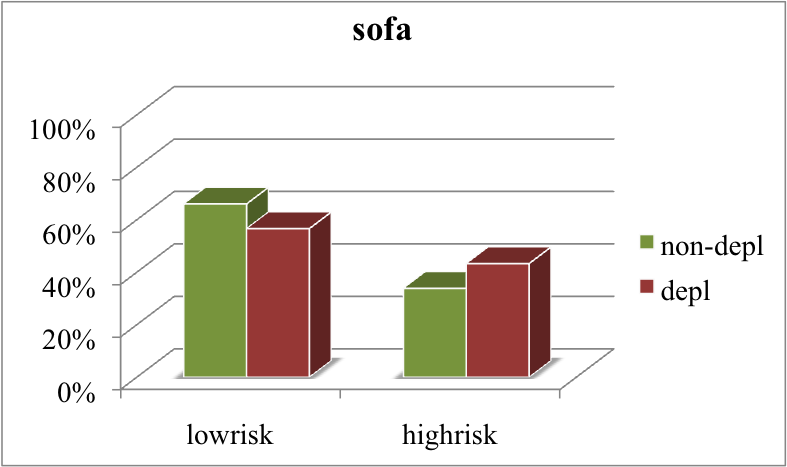
\includegraphics[trim= 1.9cm 1.2cm 2.9cm 1.43cm,clip=true,width=180pt]{images/chart_sofa}};
		\draw (-3.3,-1.9) node[anchor=east](A){0\%} ++(0,\ysep) node[anchor=east](B){20\%} ++(0,\ysep) node[anchor=east](C){40\%} ++(0,\ysep) node[anchor=east](D){60\%} ++(0,\ysep) node[anchor=east](E){80\%} ++(0,\ysep) node[anchor=east](F){100\%};
		\draw (-1.5,-2.3) node[](A1){low risk} ++(2.8,0) node[](B1){high risk};
		\node at (-3.8,2.45) {\textnormal{(sofa)}};
	% \node [label={[label distance=1cm]30:label}] {Node};	
		  \node[shape=circle,
		    fill=nondepletiongreen,
		    inner sep= 0pt,
		    label={[yshift=-1pt]right:non-depletion},
		    minimum size = 10pt,
		    line width=0pt,text=white,font=\bfseries,
		    ] at (-1.5,2.5) {};
		  \node[shape=circle,
		    fill=depletionred,
		    inner sep= 0pt,
		    label={[yshift=-1pt]right:depletion},
		    minimum size = 10pt,
		    line width=0pt,text=white,font=\bfseries,
		    ] at (1.5,2.5) {};
		% \draw (-3.4,-3) to[grid with coordinates] (3,3);
		% draw a bounding box around tikzpicture, also could use [framed] in tikzpicture environment
		% \draw [brown] (current bounding box.south west) rectangle (current bounding box.north east);
		\end{tikzpicture}
  % \rule{3cm}{3cm}%
}{%
  \caption{Ratio of participant decisions concerning ‘lowrisk’ and ‘highrisk’ in relation to non-depletion (green) and depletion (red). The ordinate denotes the share of a scale 0 to 100\%. The abscissa denotes the attribute ‘lowrisk’ and ‘highrisk’ (sofa).}\label{fig:chart_sofa}%
}
\end{floatrow}
\end{figure}
Results regarding the product ‘wine label’ indicate no statistically significant relationship between depletion and social risk (\res{Pearson chi\textsuperscript{2}(1)  = 0.0068; p  = 0.934}). In this case, abso-lutely no difference between depletion and non-depletion group emerged. In both groups 93\% opted for low risk and 7\% for high risk.

\begin{figure}[!h]
\begin{floatrow}
\capbtabbox{%
	\begin{tabu} spread 0pt {r|X[1,c] X[1,c]| c }\toprule
Wine label &   lowrisk &  highrisk &     Total\\ \midrule
  non-depl &        52 &         4 &        56 \\
      depl &        28 &         2 &        30 \\ \midrule
     Total &        80 &         6 &        86 \\  \bottomrule
	\end{tabu}\vspace{8pt}
	\begin{tabu} spread 0pt {c}
	Pearson chi\textsuperscript{2}(1) =   0.0068  Pr = 0.934
	\end{tabu}
}{%
  \caption{Results of the chi-squared test in regard to ‘social risk’ and the ‘depletion’/‘non-depletion’ condition (wine label).}\label{tab:chi_wine}%
}
\capbfigbox{%

		\begin{tikzpicture}[text depth=3pt]
		\def\ysep{0.68}
		\tikzstyle{every node}=[style={font=\footnotesize\vphantom{Ag}}]
		% trim = l b r t
		\node at (0,0) {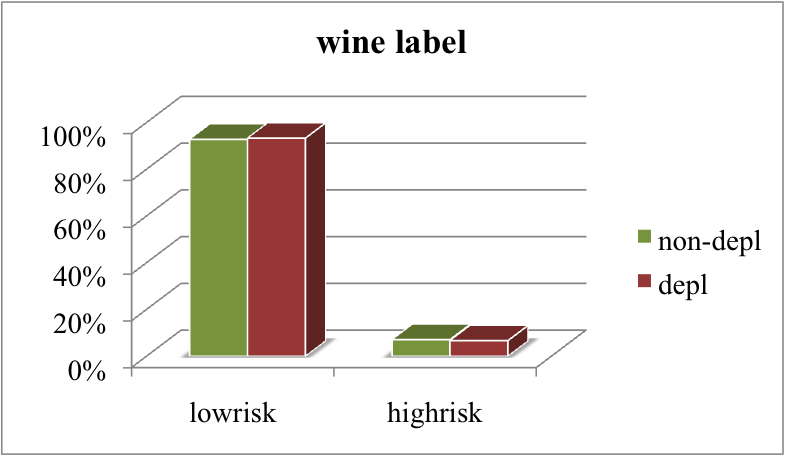
\includegraphics[trim= 2.1cm 1.35cm 3.35cm 1.6cm,clip=true,width=180pt]{images/chart_wine}};
		\draw (-3.3,-1.9) node[anchor=east](A){0\%} ++(0,\ysep) node[anchor=east](B){20\%} ++(0,\ysep) node[anchor=east](C){40\%} ++(0,\ysep) node[anchor=east](D){60\%} ++(0,\ysep) node[anchor=east](E){80\%} ++(0,\ysep) node[anchor=east](F){100\%};
		\draw (-1.5,-2.3) node[](A1){low risk} ++(2.8,0) node[](B1){high risk};
		\node at (-3.3,2.45) {\textnormal{(wine label)}};
	% \node [label={[label distance=1cm]30:label}] {Node};	
		  \node[shape=circle,
		    fill=nondepletiongreen,
		    inner sep= 0pt,
		    label={[yshift=-1pt]right:non-depletion},
		    minimum size = 10pt,
		    line width=0pt,text=white,font=\bfseries,
		    ] at (-1.5,2.5) {};
		  \node[shape=circle,
		    fill=depletionred,
		    inner sep= 0pt,
		    label={[yshift=-1pt]right:depletion},
		    minimum size = 10pt,
		    line width=0pt,text=white,font=\bfseries,
		    ] at (1.5,2.5) {};
		% \draw (-3,-3) to[grid with coordinates] (3.5,3);

		% \draw [brown] (current bounding box.south west) rectangle (current bounding box.north east);
		\end{tikzpicture}
  % \rule{3cm}{3cm}%
}{%
  \caption{Ratio of participant decisions concerning ‘lowrisk’ and ‘highrisk’ in relation to non-depletion (green) and deple-tion (red). The ordinate denotes the share of a scale 0 to 100\%. The abscissa denotes the attribute ‘lowrisk’ and ‘highrisk’ (wine label).}\label{fig:chart_wine}%
}
\end{floatrow}
\end{figure}
Results regarding the product ‘car’ revealed no statistically significant relationship be-tween the type of depletion and social risk (\res{Pearson chi\textsuperscript{2}(1)  = 0.0193; p = 0.889}). Similar to ‘wine label’, both groups differ scarcely from each other. Of the non-depletion group 77\% opted for low risk, whereas 23\% opted for high risk. Of the depletion group 83\% opted for low risk as opposed to 17\% who opted for low risk. 

\begin{figure}[!h]
\begin{floatrow}
\capbtabbox{%
	\begin{tabu} spread 0pt {r|X[1,c] X[1,c]| c }\toprule
      car  &   lowrisk &  highrisk &     Total \\ \midrule
  non-depl &        40 &        16 &        56 \\
      depl &        21 &         9 &        30 \\ \midrule
     Total &        61 &        25 &        86 \\ \bottomrule
	\end{tabu}\vspace{8pt}
	\begin{tabu} spread 0pt {c}
	Pearson chi\textsuperscript{2}(1) =   0.0193  Pr = 0889.
	\end{tabu}
}{%
  \caption{Results of the chi-squared test in regard to ‘social risk’ and the ‘depletion’/‘non-depletion’ condition (car).}\label{tab:chi_car}%
}
\capbfigbox{%

		\begin{tikzpicture}[text depth=3pt]
		\def\ysep{0.68}
		\tikzstyle{every node}=[style={font=\footnotesize\vphantom{Ag}}]
		% trim = l b r t
		\node at (0,0) {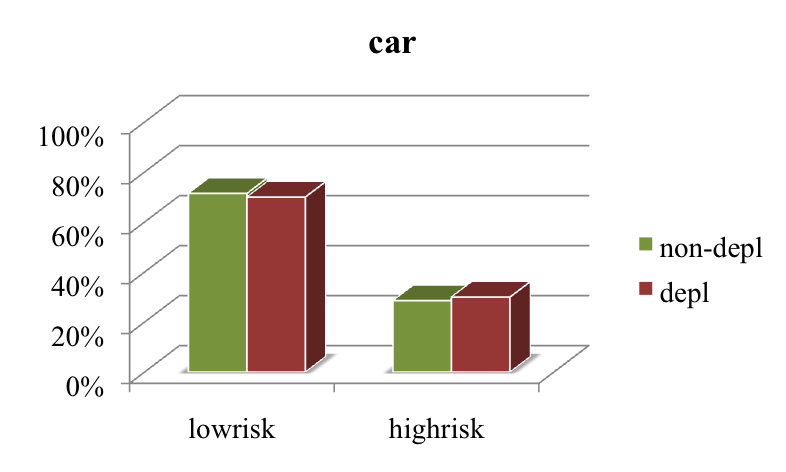
\includegraphics[trim= 2.1cm 1.35cm 3.35cm 1.6cm,clip=true,width=180pt]{images/chart_car}};
		\draw (-3.3,-1.9) node[anchor=east](A){0\%} ++(0,\ysep) node[anchor=east](B){20\%} ++(0,\ysep) node[anchor=east](C){40\%} ++(0,\ysep) node[anchor=east](D){60\%} ++(0,\ysep) node[anchor=east](E){80\%} ++(0,\ysep) node[anchor=east](F){100\%};
		\draw (-1.5,-2.3) node[](A1){low risk} ++(2.8,0) node[](B1){high risk};
		\node at (-3.8,2.45) {\textnormal{(car)}};
	% \node [label={[label distance=1cm]30:label}] {Node};	
		  \node[shape=circle,
		    fill=nondepletiongreen,
		    inner sep= 0pt,
		    label={[yshift=-1pt]right:non-depletion},
		    minimum size = 10pt,
		    line width=0pt,text=white,font=\bfseries,
		    ] at (-1.5,2.5) {};
		  \node[shape=circle,
		    fill=depletionred,
		    inner sep= 0pt,
		    label={[yshift=-1pt]right:depletion},
		    minimum size = 10pt,
		    line width=0pt,text=white,font=\bfseries,
		    ] at (1.5,2.5) {};
		% \draw (-3,-3) to[grid with coordinates] (3.5,3);
		\end{tikzpicture}
  % \rule{3cm}{3cm}%
}{%
  \caption{Ratio of participant decisions concerning ‘lowrisk’ and ‘highrisk’ in relation to non-depletion (green) and depletion (red). The ordinate denotes the share of a scale 0 to 100\%. The abscissa denotes the attribute ‘lowrisk’ and ‘highrisk’ (car).}\label{fig:chart_car}%
}
\end{floatrow}
\end{figure}
Results regarding the product ‘mp3 player’ revealed no statistically significant relationship between depletion and social risk (\res{Pearson chi\textsuperscript{2}(1)  = 0.0506; p = 0.477}). Nevertheless, results indicate a slightly stronger tendency within the depletion group to favor the low risk alternative compared to non-depleted participants. Still, the difference is clearly too minor to reach a significant level. 

\begin{figure}[!h]
\begin{floatrow}
\capbtabbox{%
	\begin{tabu} spread 0pt {r|X[1,c] X[1,c]| c }\toprule
mp3 player &   lowrisk&   highrisk &     Total \\  \midrule
  non-depl &        43&         13 &        56 \\
      depl &        25&          5 &        30 \\   \midrule
     Total &        68&         18 &        86 \\   \bottomrule
	\end{tabu}\vspace{8pt}
	\begin{tabu} spread 0pt {c}
	Pearson chi\textsuperscript{2}(1) =   0.5060  Pr = 0.447
	\end{tabu}
}{%
  \caption{Results of the chi-squared test in regard to ‘social risk’ and the ‘depletion’/‘non-depletion’ condition (mp3 player).}\label{tab:chi_mp3}%
}
\capbfigbox{%

		\begin{tikzpicture}[text depth=3pt]
		\def\ysep{0.68}
		\tikzstyle{every node}=[style={font=\footnotesize\vphantom{Ag}}]
		% trim = l b r t
		\node at (0,0) {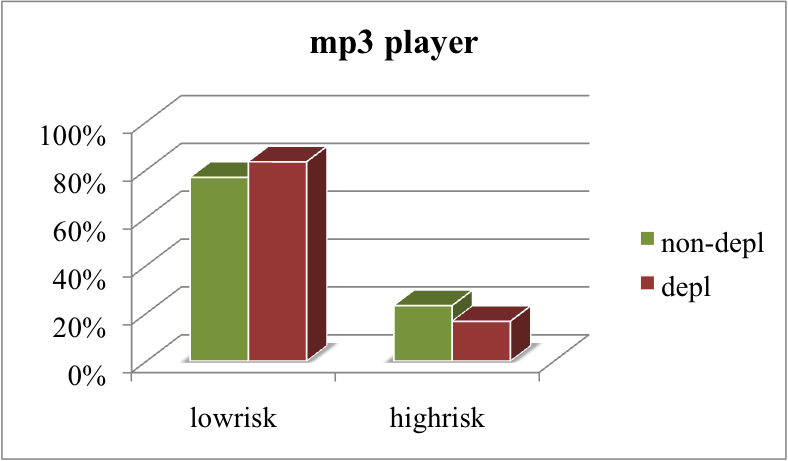
\includegraphics[trim= 2.1cm 1.35cm 3.35cm 1.6cm,clip=true,width=180pt]{images/chart_mp3}};
		\draw (-3.3,-1.9) node[anchor=east](A){0\%} ++(0,\ysep) node[anchor=east](B){20\%} ++(0,\ysep) node[anchor=east](C){40\%} ++(0,\ysep) node[anchor=east](D){60\%} ++(0,\ysep) node[anchor=east](E){80\%} ++(0,\ysep) node[anchor=east](F){100\%};
		\draw (-1.5,-2.3) node[](A1){low risk} ++(2.8,0) node[](B1){high risk};
		\node at (-3.3,2.45) {\textnormal{(mp3 player)}};
	% \node [label={[label distance=1cm]30:label}] {Node};	
		  \node[shape=circle,
		    fill=nondepletiongreen,
		    inner sep= 0pt,
		    label={[yshift=-1pt]right:non-depletion},
		    minimum size = 10pt,
		    line width=0pt,text=white,font=\bfseries,
		    ] at (-1.5,2.5) {};
		  \node[shape=circle,
		    fill=depletionred,
		    inner sep= 0pt,
		    label={[yshift=-1pt]right:depletion},
		    minimum size = 10pt,
		    line width=0pt,text=white,font=\bfseries,
		    ] at (1.5,2.5) {};
		% \draw (-3,-3) to[grid with coordinates] (3.5,3);
		\end{tikzpicture}
  % \rule{3cm}{3cm}%
}{%
  \caption{Ratio of participant decisions concerning ‘lowrisk’ and ‘highrisk’ in relation to non-depletion (green) and depletion (red). The ordinate denotes the share of a scale 0 to 100\%. The abscissa denotes the attribute ‘lowrisk’ and ‘highrisk’ (mp3 player)}\label{fig:chart_mp3}%
}
\end{floatrow}
\end{figure}
Results regarding the product ‘shoes’ revealed no statistically significant relationship be-tween the type of depletion and social risk (\res{Pearson chi\textsuperscript{2}(1)  = 0.1223, p = 0.727}). Consistent with the results obtained for ‘mp3-player’, results indicate a slightly stronger tendency within the depletion group to favor the low risk alternative compared to non-depleted participants, again, not enough to reach significance.

\begin{figure}[!h]
\begin{floatrow}
\capbtabbox{%
	\begin{tabu} spread 0pt {r|X[1,c] X[1,c]| c }\toprule
     shoes &   lowrisk &  highrisk &     Total \\  \midrule
  non-depl &        41 &        15 &        56 \\
      depl &        23 &         7 &        30 \\  \midrule
     Total &        64 &        22 &        86 \\  \bottomrule
	\end{tabu}\vspace{8pt}
	\begin{tabu} spread 0pt {c}
	Pearson chi\textsuperscript{2}(1) =   0.1223  Pr = 0.727
	\end{tabu}
}{%
  \caption{Results of the chi-squared test in regard to ‘social risk’ and the ‘depletion’/‘non-depletion’ condition (shoes).}\label{tab:chi_shoes}%
}
\capbfigbox{%

		\begin{tikzpicture}[text depth=3pt]
		\def\ysep{0.68}
		\tikzstyle{every node}=[style={font=\footnotesize\vphantom{Ag}}]
		% trim = l b r t
		\node at (0,0) {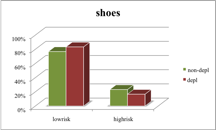
\includegraphics[trim= 2.1cm 1.35cm 3.35cm 1.6cm,clip=true,width=180pt]{images/chart_shoes}};
		\draw (-3.3,-1.9) node[anchor=east](A){0\%} ++(0,\ysep) node[anchor=east](B){20\%} ++(0,\ysep) node[anchor=east](C){40\%} ++(0,\ysep) node[anchor=east](D){60\%} ++(0,\ysep) node[anchor=east](E){80\%} ++(0,\ysep) node[anchor=east](F){100\%};
		\draw (-1.5,-2.3) node[](A1){low risk} ++(2.8,0) node[](B1){high risk};
		\node at (-3.7,2.45) {\textnormal{(shoes)}};
	% \node [label={[label distance=1cm]30:label}] {Node};	
		  \node[shape=circle,
		    fill=nondepletiongreen,
		    inner sep= 0pt,
		    label={[yshift=-1pt]right:non-depletion},
		    minimum size = 10pt,
		    line width=0pt,text=white,font=\bfseries,
		    ] at (-1.5,2.5) {};
		  \node[shape=circle,
		    fill=depletionred,
		    inner sep= 0pt,
		    label={[yshift=-1pt]right:depletion},
		    minimum size = 10pt,
		    line width=0pt,text=white,font=\bfseries,
		    ] at (1.5,2.5) {};
		% \draw (-3,-3) to[grid with coordinates] (3.5,3);
		\end{tikzpicture}
  % \rule{3cm}{3cm}%
}{%
  \caption{Ratio of participant decisions concerning ‘lowrisk’ and ‘highrisk’ in relation to non-depletion (green) and depletion (red). The ordinate denotes the share of a scale 0 to 100\%. The abscissa denotes the attribute ‘lowrisk’ and ‘highrisk’ (shoes).}\label{fig:chart_shoes}%
}
\end{floatrow}
\end{figure}
Summing up, results of the chi-squared tests revealed that our initial assumption (depleted participants opt in favor of products involving a low social risk) was not only incorrect but also revealed opposing results for one out of five products that were tested, namely the sofa. The other products did not reveal any significant data to support our assumption (\res{chi\textsuperscript{2} = 0.7395 (sofa) vs. chi\textsuperscript{2} = 0.0068 (wine label); 0.0193 (car); 0.0506 (mp3-player); 0.1223 (shoes)}), even if a slightly stronger tendency to prefer the low risk alternative was present for ‘mp3-player’ and ‘shoes’ within the depletion group compared to the non-depletion group.\par
\FloatBarrier
\subsection{Pearson Chi-Squared Test (Judges’ Dilemma)}\label{sec:pearson_chi_judges}
Results regarding the judges’ case 1 indicate no statistically significant relationship be-tween depletion and social risk emerged (\res{Pearson chi\textsuperscript{2}(1)  = 0.1262, p = 0.722}). Consistent with the results obtained for ‘shoes’ and ‘mp3-player’, results indicate a slightly stronger tendency within the depletion group to favor the low risk alternative compared to non-depleted participants. Also consistent with the products, levels of difference did not reach significance.

\begin{figure}[!h]
\begin{floatrow}
\capbtabbox{%
	\begin{tabu} spread 0pt {r|X[1,c] X[1.3,c]| c }\toprule
  Judge1   &   custody&  probation &     Total \\  \midrule
  non-depl &        43&         13 &        56 \\
      depl &        22&          8 &        30 \\    \midrule
     Total &        65&         21 &        86 \\    \bottomrule
	\end{tabu}\vspace{8pt}
	\begin{tabu} spread 0pt {c}
	Pearson chi\textsuperscript{2}(1) =   0.1262  Pr = 0.722
	\end{tabu}
}{%
  \caption{Results of the chi-squared test in regard to ‘social risk’ and the ‘depletion’/‘non-depletion’ condition (judges’ case 1).}\label{tab:chi_judges1}%
}
\capbfigbox{%

		\begin{tikzpicture}[text depth=3pt]
		\def\ysep{0.68}
		\tikzstyle{every node}=[style={font=\footnotesize\vphantom{Ag}}]
		% trim = l b r t
		\node at (0,0) {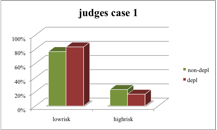
\includegraphics[trim= 2.1cm 1.35cm 3.35cm 1.6cm,clip=true,width=180pt]{images/chart_JD1}};
		\draw (-3.3,-1.9) node[anchor=east](A){0\%} ++(0,\ysep) node[anchor=east](B){20\%} ++(0,\ysep) node[anchor=east](C){40\%} ++(0,\ysep) node[anchor=east](D){60\%} ++(0,\ysep) node[anchor=east](E){80\%} ++(0,\ysep) node[anchor=east](F){100\%};
		\draw (-1.5,-2.3) node[](A1){low risk} ++(2.8,0) node[](B1){high risk};
		\node at (-3.1,2.45) {\textnormal{(judges’ case 1)}};
	% \node [label={[label distance=1cm]30:label}] {Node};	
		  \node[shape=circle,
		    fill=nondepletiongreen,
		    inner sep= 0pt,
		    label={[yshift=-1pt]right:non-depletion},
		    minimum size = 10pt,
		    line width=0pt,text=white,font=\bfseries,
		    ] at (-1.5,2.5) {};
		  \node[shape=circle,
		    fill=depletionred,
		    inner sep= 0pt,
		    label={[yshift=-1pt]right:depletion},
		    minimum size = 10pt,
		    line width=0pt,text=white,font=\bfseries,
		    ] at (1.5,2.5) {};
		% \draw (-3,-3) to[grid with coordinates] (3.5,3);
		\end{tikzpicture}
  % \rule{3cm}{3cm}%
}{%
  \caption{Ratio of participant decisions concerning ‘lowrisk’ and ‘highrisk’ in relation to non-depletion (green) and depletion (red). The ordinate denotes the share of a scale 0 to 100\%. The abscissa denotes the attribute ‘lowrisk’ and ‘highrisk’ (judges’ case 1).}\label{fig:chart_judges1}%
}
\end{floatrow}
\end{figure}

Results regarding the judges’ case 2 revealed no statistically significant relationship be-tween the type of depletion and social risk (\res{Pearson chi\textsuperscript{2}(1)  = 0.0999, p = 0.752}). Again, results indicate a slightly stronger tendency within the depletion group to favor the low risk alternative compared to non-depleted participants but did not reach a significant level.\par

\begin{figure}[!h]
\begin{floatrow}
\capbtabbox{%
	\begin{tabu} spread 0pt {r|X[1,c] X[1.3,c]| c }\toprule
  Judge2   &   custody&  probation &     Total \\  \midrule
  non-depl &        26&         30 &        56 \\
      depl &        15&         15 &        30 \\   \midrule
     Total &        41&         45 &        86 \\   \bottomrule
	\end{tabu}\vspace{8pt}
	\begin{tabu} spread 0pt {c}
	Pearson chi\textsuperscript{2}(1) =   0.0999  Pr = 0.752
	\end{tabu}
}{%
  \caption{Results of the chi-squared test in regard to ‘social risk’ and the ‘depletion’/‘non-depletion’ condition (judges’ case 2).}\label{tab:chi_judges2}%
}
\capbfigbox{%

		\begin{tikzpicture}[text depth=3pt]
		\def\ysep{0.68}
		\tikzstyle{every node}=[style={font=\footnotesize\vphantom{Ag}}]
		% trim = l b r t
		\node at (0,0) {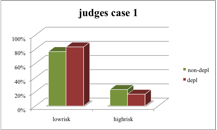
\includegraphics[trim= 2.1cm 1.35cm 3.35cm 1.6cm,clip=true,width=180pt]{images/chart_JD1}};
		\draw (-3.3,-1.9) node[anchor=east](A){0\%} ++(0,\ysep) node[anchor=east](B){20\%} ++(0,\ysep) node[anchor=east](C){40\%} ++(0,\ysep) node[anchor=east](D){60\%} ++(0,\ysep) node[anchor=east](E){80\%} ++(0,\ysep) node[anchor=east](F){100\%};
		\draw (-1.5,-2.3) node[](A1){low risk} ++(2.8,0) node[](B1){high risk};
		\node at (-3.1,2.45) {\textnormal{(judges’ case 2)}};
	% \node [label={[label distance=1cm]30:label}] {Node};	
		  \node[shape=circle,
		    fill=nondepletiongreen,
		    inner sep= 0pt,
		    label={[yshift=-1pt]right:non-depletion},
		    minimum size = 10pt,
		    line width=0pt,text=white,font=\bfseries,
		    ] at (-1.5,2.5) {};
		  \node[shape=circle,
		    fill=depletionred,
		    inner sep= 0pt,
		    label={[yshift=-1pt]right:depletion},
		    minimum size = 10pt,
		    line width=0pt,text=white,font=\bfseries,
		    ] at (1.5,2.5) {};
		% \draw (-3,-3) to[grid with coordinates] (3.5,3);
		\end{tikzpicture}
  % \rule{3cm}{3cm}%
}{%
  \caption{Ratio of participant decisions concerning ‘lowrisk’ and ‘highrisk’ in relation to non-depletion (green) and deple-tion (red). The ordinate denotes the share of a scale 0 to 100\%. The abscissa denotes the attribute ‘lowrisk’ and ‘highrisk’ (judges’ case 2).}\label{fig:chart_judges2}%
}
\end{floatrow}
\end{figure}
Results regarding the judges’ case 3 revealed no statistically significant relationship be-tween condition and social risk (\res{Pearson chi\textsuperscript{2}(1)  = 1.620; p = 0.281}), however, the result again contradicted our assumption. In this case 71\% of the non-depletion condition group opted for low risk, whereas 29\% opted for high risk. In the depletion condition group 60\% of the participants opted for low risk, whereas 40\% opted for high risk. As expected, both groups showed a clear preference for the low risk alternative although this preference was more pro-nounced within the non-depletion condition.\par

\begin{figure}[!h]
\begin{floatrow}
\capbtabbox{%
	\begin{tabu} spread 0pt {r|X[1,c] X[1.3,c]| c }\toprule
    Judge3 &   custody&  probation &     Total \\   \midrule
  non-depl &        40&         16 &        56 \\
      depl &        18&         12 &        30 \\  \midrule
     Total &        58&         28 &        86 \\   \bottomrule
	\end{tabu}\vspace{8pt}
	\begin{tabu} spread 0pt {c}
	Pearson chi\textsuperscript{2}(1) =   1.1620  Pr = 0.281
	\end{tabu}
}{%
  \caption{Results of the chi-squared test in regard to ‘social risk’ and the ‘depletion’/‘non-depletion’ condition (judges’ case 3).}\label{tab:chi_judges3}%
}
\capbfigbox{%

		\begin{tikzpicture}[text depth=3pt]
		\def\ysep{0.68}
		\tikzstyle{every node}=[style={font=\footnotesize\vphantom{Ag}}]
		% trim = l b r t
		\node at (0,0) {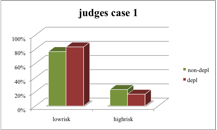
\includegraphics[trim= 2.1cm 1.35cm 3.35cm 1.6cm,clip=true,width=180pt]{images/chart_JD1}};
		\draw (-3.3,-1.9) node[anchor=east](A){0\%} ++(0,\ysep) node[anchor=east](B){20\%} ++(0,\ysep) node[anchor=east](C){40\%} ++(0,\ysep) node[anchor=east](D){60\%} ++(0,\ysep) node[anchor=east](E){80\%} ++(0,\ysep) node[anchor=east](F){100\%};
		\draw (-1.5,-2.3) node[](A1){low risk} ++(2.8,0) node[](B1){high risk};
		\node at (-3.1,2.45) {\textnormal{(judges’ case 3)}};
	% \node [label={[label distance=1cm]30:label}] {Node};	
		  \node[shape=circle,
		    fill=nondepletiongreen,
		    inner sep= 0pt,
		    label={[yshift=-1pt]right:non-depletion},
		    minimum size = 10pt,
		    line width=0pt,text=white,font=\bfseries,
		    ] at (-1.5,2.5) {};
		  \node[shape=circle,
		    fill=depletionred,
		    inner sep= 0pt,
		    label={[yshift=-1pt]right:depletion},
		    minimum size = 10pt,
		    line width=0pt,text=white,font=\bfseries,
		    ] at (1.5,2.5) {};
		% \draw (-3,-3) to[grid with coordinates] (3.5,3);
		\end{tikzpicture}
  % \rule{3cm}{3cm}%
}{%
  \caption{Ratio of participant decisions concerning ‘lowrisk’ and ‘highrisk’ in relation to non-depletion (green) and depletion (red). The ordinate denotes the share of a scale 0 to 100\%. The abscissa denotes the attribute ‘lowrisk’ and ‘highrisk’ (judges’ case 3).}\label{fig:chart_judges2}%
}
\end{floatrow}
\end{figure}
Summing up, results of the chi-squared tests revealed that our initial assumption (depleted participants opt in favor of verdicts involving a low social risk) was not only incorrect but also revealed opposing results for one out of three cases that were tested, videlicet judges’ case 3. The other cases did not reveal any significant data to support our assumption (\res{chi\textsuperscript{2} = 1.1620 (Judge3) vs. chi\textsuperscript{2}  = 0.1262 (Judge1); 0.0999 (Judge2)}), even if a slightly stronger tendency to prefer the low risk alternative was present for ‘Judge1’ and ‘Judge2’ within the depletion group compared to the non-depletion group.\par

\FloatBarrier
\section{Examination of Depletion, and Self-Evaluation with regard to Difficulty and Exhaustion}\label{sec:depletion_measure_selfevaluation}
Figure 17 displays the ratio of correct answers given by the experimental group and the control group in the cognitive reflection test (see Section \ref{sec:judgeschoice}). The results show that 30\% of the non-depletion group and nearly 30\% of the depletion group did not manage to provide at least one correct answer. 37\% of the depletion group and approximately 17\% of the non-depletion group provided one correct answer. The number of participants in both groups de-clined with the rising number of correct answers. However, the non-depletion group was relatively stronger to answer more correct question then the depletion group. \par
A two-sample t-test with equal variances was administered in order assert that the deple-tion task affected participants in the experimental group. Results revealed that the experimental group answered less questions correctly compared to the control group with the non-depleting Stroop test (\res{t = 1.33; df = 84; p = 0.188}). Therefore, it can be assumed that the Stroop test did deplete the experimental group. \par
\begin{figure}[h!]
		\begin{tikzpicture}[text depth=3pt]
		\def\ysep{0.87}
		\tikzstyle{every node}=[style={font=\footnotesize\vphantom{Ag}}]
		% trim = l b r t
		\node at (0,0) {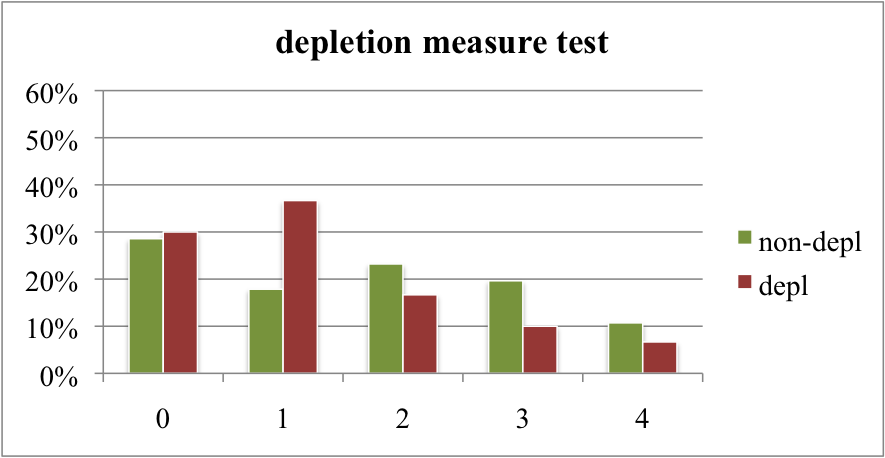
\includegraphics[trim= 2.1cm 1.35cm 3.35cm 1.5cm,clip=true,width=290pt]{images/chart_depletion_measure}};
		\draw (-5.5,-2.6) node[anchor=east](A){0\%} ++(0,\ysep) node[anchor=east](B){10\%} ++(0,\ysep) node[anchor=east](C){20\%} ++(0,\ysep) node[anchor=east](D){30\%} ++(0,\ysep) node[anchor=east](E){40\%} ++(0,\ysep) node[anchor=east](F){50\%}++(0,\ysep) node[anchor=east](G){60\%};
		\def\xsep{2.25}
		\draw (-4.57,-3) node[](A1){1} ++(\xsep,0) node[](B1){2} ++(\xsep,0) node[](C1){3} ++(\xsep,0) node[](D1){4} ++(\xsep,0) node[](E1){5};
		\node at (-2.7,2.28) {\textnormal{(depletion measure)}};
		  \node[shape=circle,
		    fill=nondepletiongreen,
		    inner sep= 0pt,
		    label={[yshift=-1pt]right:non-depletion},
		    minimum size = 10pt,
		    line width=0pt,text=white,font=\bfseries,
		    ] at (-0.9,2.29) {};
		  \node[shape=circle,
		    fill=depletionred,
		    inner sep= 0pt,
		    label={[yshift=-1pt]right:depletion},
		    minimum size = 10pt,
		    line width=0pt,text=white,font=\bfseries,
		    ] at (2.2,2.29) {};
		% \draw (-6,-3) to[grid with coordinates] (6,3);
		\end{tikzpicture}
		\vspace{-12pt}
		\caption{Ratio of correct answers in the depletion task regarding to non-depletion and depletion. The ordinate denotes the share of participants on a scale from 0 to 60\%. The abscissa denotes the number of correct answers.}\label{fig:chart_depletion_measure}
\end{figure}
\begin{figure}[h!]
		\begin{tikzpicture}[text depth=3pt]
		\def\ysep{0.87}
		\tikzstyle{every node}=[style={font=\footnotesize\vphantom{Ag}}]
		% trim = l b r t
		\node at (0,0) {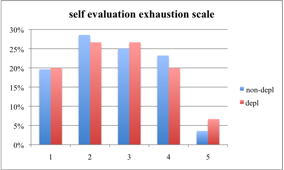
\includegraphics[trim= 2.1cm 1.35cm 3.35cm 1.5cm,clip=true,width=290pt]{images/chart_se_exhaustion}};
		\draw (-5.5,-2.6) node[anchor=east](A){0\%} ++(0,\ysep) node[anchor=east](B){10\%} ++(0,\ysep) node[anchor=east](C){20\%} ++(0,\ysep) node[anchor=east](D){30\%} ++(0,\ysep) node[anchor=east](E){40\%} ++(0,\ysep) node[anchor=east](F){50\%}++(0,\ysep) node[anchor=east](G){60\%};
		\def\xsep{2.25}
		\draw (-4.57,-3) node[](A1){1} ++(\xsep,0) node[](B1){2} ++(\xsep,0) node[](C1){3} ++(\xsep,0) node[](D1){4} ++(\xsep,0) node[](E1){5};
		\node at (-2.7,2.28) {\textnormal{(depletion measure)}};
		  \node[shape=circle,
		    fill=nondepletiongreen,
		    inner sep= 0pt,
		    label={[yshift=-1pt]right:non-depletion},
		    minimum size = 10pt,
		    line width=0pt,text=white,font=\bfseries,
		    ] at (-0.9,2.29) {};
		  \node[shape=circle,
		    fill=depletionred,
		    inner sep= 0pt,
		    label={[yshift=-1pt]right:depletion},
		    minimum size = 10pt,
		    line width=0pt,text=white,font=\bfseries,
		    ] at (2.2,2.29) {};
		% \draw (-3,-3) to[grid with coordinates] (3.5,3);
		\end{tikzpicture}
		\vspace{-12pt}
		\caption{Ratio of self evaluation ‘exhaustion’ regarding to non-depletion and depletion. The ordinate denotes the share of participants on a scale from 0 to 60\%. The abscissa denotes the scale ‘exhaustion’ from one to five.}\label{fig:self_evaluation_exhaustion_scale}
\end{figure}
\begin{figure}[H]
		\begin{tikzpicture}[text depth=3pt]
		\def\ysep{0.87}
		\tikzstyle{every node}=[style={font=\footnotesize\vphantom{Ag}}]
		\node at (0,0) {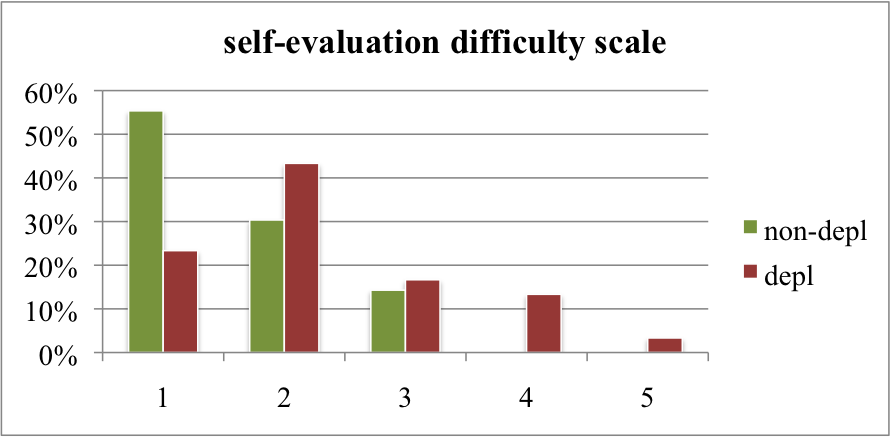
\includegraphics[trim= 2.1cm 1.3cm 3.35cm 1.5cm,clip=true, height=150pt,width=290pt]{images/chart_se_difficulty}};
		\draw (-5.5,-2.6) node[anchor=east](A){0\%} ++(0,\ysep) node[anchor=east](B){10\%} ++(0,\ysep) node[anchor=east](C){20\%} ++(0,\ysep) node[anchor=east](D){30\%} ++(0,\ysep) node[anchor=east](E){40\%} ++(0,\ysep) node[anchor=east](F){50\%}++(0,\ysep) node[anchor=east](G){60\%};
		\def\xsep{2.25}
		\draw (-4.57,-3) node[](A1){1} ++(\xsep,0) node[](B1){2} ++(\xsep,0) node[](C1){3} ++(\xsep,0) node[](D1){4} ++(\xsep,0) node[](E1){5};
		\node at (-2.7,2.28) {\textnormal{(depletion measure)}};
		  \node[shape=circle,
		    fill=nondepletiongreen,
		    inner sep= 0pt,
		    label={[yshift=-1pt]right:non-depletion},
		    minimum size = 10pt,
		    line width=0pt,text=white,font=\bfseries,
		    ] at (-0.9,2.29) {};
		  \node[shape=circle,
		    fill=depletionred,
		    inner sep= 0pt,
		    label={[yshift=-1pt]right:depletion},
		    minimum size = 10pt,
		    line width=0pt,text=white,font=\bfseries,
		    ] at (2.2,2.29) {};
		% trim = l b r t
		% \draw (-3,-3) to[grid with coordinates] (3.5,3);
		\end{tikzpicture}
		\vspace{-12pt}
		\caption{Ratio of self evaluation ‘difficulty’ regarding to non-depletion and depletion. The ordinate denotes the share of participants on a scale from 0 to 60\%. The abscissa denotes the scale ‘difficulty’ ranging from one to five.}\label{fig:self_evaluation_difficulty_scale}
\end{figure}
After completing the depletion measure test participants of both groups were asked to rate their personal level of exhaustion and their perceived level of difficulty of the questionnaire on a Likert scale ranging from 1 (not at all exhausted / very easy) to 5 (very exhausted / very difficult) (see Section \ref{sec:depletionself-evaluation}). According to Figure 18 it appears that participants in the depletion condition did not feel remarkably more exhausted than participants in the non-depletion condition. Nevertheless, Figure 19 reveals that depleted participants rated the difficulty of the questionnaire higher than non-depleted participants, which supports the assumptions drawn from the depletion measure test. \par